%%%%%%%%%%%%%%%%%%%%%%%%%%%%%%%%%%%%%%%%%
% Masters/Doctoral Thesis 
% LaTeX Template
% Version 2.5 (27/8/17)
%
% This template was downloaded from:
% http://www.LaTeXTemplates.com
%
% Version 2.x major modifications by:
% Vel (vel@latextemplates.com)
%
% This template is based on a template by:
% Steve Gunn (http://users.ecs.soton.ac.uk/srg/softwaretools/document/templates/)
% Sunil Patel (http://www.sunilpatel.co.uk/thesis-template/)
%
% Template license:
% CC BY-NC-SA 3.0 (http://creativecommons.org/licenses/by-nc-sa/3.0/)
%
%%%%%%%%%%%%%%%%%%%%%%%%%%%%%%%%%%%%%%%%%

%----------------------------------------------------------------------------------------
%	PACKAGES AND OTHER DOCUMENT CONFIGURATIONS
%----------------------------------------------------------------------------------------

\documentclass[
12pt, % The default document font size, options: 10pt, 11pt, 12pt
oneside, % Two side (alternating margins) for binding by default, uncomment to switch to one side
english, % ngerman for German
onehalfspacing, % Single line spacing, alternatives: onehalfspacing or doublespacing
%draft, % Uncomment to enable draft mode (no pictures, no links, overfull hboxes indicated)
%nolistspacing, % If the document is onehalfspacing or doublespacing, uncomment this to set spacing in lists to single
%liststotoc, % Uncomment to add the list of figures/tables/etc to the table of contents
%toctotoc, % Uncomment to add the main table of contents to the table of contents
%parskip, % Uncomment to add space between paragraphs
%nohyperref, % Uncomment to not load the hyperref package
headsepline, % Uncomment to get a line under the header
%chapterinoneline, % Uncomment to place the chapter title next to the number on one line
%consistentlayout, % Uncomment to change the layout of the declaration, abstract and acknowledgements pages to match the default layout
]{MastersDoctoralThesis} % The class file specifying the document structure

\usepackage[utf8]{inputenc} % Required for inputting international characters
\usepackage[T1]{fontenc} % Output font encoding for international characters
\usepackage{todonotes}
\usepackage{mathpazo} % Use the Palatino font by default

%\usepackage[style=numeric]{biblatex} % Use the bibtex backend with the authoryear citation style (which resembles APA)
\usepackage[backend=bibtex,style=numeric]{biblatex}
\bibliography{main} 
	
\usepackage[autostyle=true]{csquotes} % Required to generate language-dependent quotes in the bibliography

%----------------------------------------------------------------------------------------
%	MARGIN SETTINGS
%----------------------------------------------------------------------------------------

\geometry{
	paper=a4paper, % Change to letterpaper for US letter
	inner=2.5cm, % Inner margin`
	outer=3.8cm, % Outer margin
	bindingoffset=.5cm, % Binding offset
	top=1.5cm, % Top margin
	bottom=1.5cm, % Bottom margin
	%showframe, % Uncomment to show how the type block is set on the page
}

%----------------------------------------------------------------------------------------
%	THESIS INFORMATION
%----------------------------------------------------------------------------------------

\thesistitle{low cost biomedical device platform with a parameter SPO2} % Your thesis title, this is used in the title and abstract, print it elsewhere with \ttitle
\supervisor{Dr. Paul \textsc{Gardner-Stephen}} % Your supervisor's name, this is used in the title page, print it elsewhere with \supname
\examiner{} % Your examiner's name, this is not currently used anywhere in the template, print it elsewhere with \examname
\degree{Master of Engineering(Biomedical)} % Your degree name, this is used in the title page and abstract, print it elsewhere with \degreename
\author{Thomas Thomas} % Your name, this is used in the title page and abstract, print it elsewhere with \authorname
\addresses{} % Your address, this is not currently used anywhere in the template, print it elsewhere with \addressname

\subject{Biomedical Engineering} % Your subject area, this is not currently used anywhere in the template, print it elsewhere with \subjectname
\keywords{} % Keywords for your thesis, this is not currently used anywhere in the template, print it elsewhere with \keywordnames
\university{\href{https://www.flinders.edu.au/}{Flinders University}} % Your university's name and URL, this is used in the title page and abstract, print it elsewhere with \univname
\department{\href{https://www.flinders.edu.au/college-science-engineering}{College of Science and Engineering}} % Your department's name and URL, this is used in the title page and abstract, print it elsewhere with \deptname
\group{The Douglas Adams Institute For Implausible Linguistics} % Your research group's name and URL, this is used in the title page, print it elsewhere with \groupname
\faculty{\href{}{}} % Your faculty's name and URL, this is used in the title page and abstract, print it elsewhere with \facname

\AtBeginDocument{
\hypersetup{pdftitle=\ttitle} % Set the PDF's title to your title
\hypersetup{pdfauthor=\authorname} % Set the PDF's author to your name
\hypersetup{pdfkeywords=\keywordnames} % Set the PDF's keywords to your keywords
}

\begin{document}

\frontmatter % Use roman page numbering style (i, ii, iii, iv...) for the pre-content pages

\pagestyle{plain} % Default to the plain heading style until the thesis style is called for the body content

%----------------------------------------------------------------------------------------
%	TITLE PAGE
%----------------------------------------------------------------------------------------

\begin{titlepage}
\begin{center}

\vspace*{.06\textheight}
{\scshape\LARGE \univname\par}\vspace{1.5cm} % University name
\textsc{\Large Master Thesis}\\[0.5cm] % Thesis type

\HRule \\[0.4cm] % Horizontal line
{\huge \bfseries \ttitle\par}\vspace{0.4cm} % Thesis title
\HRule \\[1.5cm] % Horizontal line
 
\begin{minipage}[t]{0.4\textwidth}
\begin{flushleft} \large
\emph{Author:}\\
{\authorname} % Author name - remove the \href bracket to remove the link
\end{flushleft}
\end{minipage}
\begin{minipage}[t]{0.4\textwidth}
\begin{flushright} \large
\emph{Supervisor:} \\
{\supname} % Supervisor name - remove the \href bracket to remove the link  
\end{flushright}
\end{minipage}\\[3cm]
 
\vfill

\large \textit{A thesis submitted in fulfilment of the requirements\\ for the degree of \degreename}\\[0.3cm] % University requirement text
%%\groupname\\\deptname\\[2cm] % Research group name and department name
 
\vfill

{\large \today}\\[4cm] % Date
%\includegraphics{Logo} % University/department logo - uncomment to place it
 
\vfill
\end{center}
\end{titlepage}

%----------------------------------------------------------------------------------------
%	DECLARATION PAGE
%----------------------------------------------------------------------------------------

\begin{declaration}
\addchaptertocentry{\authorshipname} % Add the declaration to the table of contents
\noindent I, \authorname, declare that this thesis titled, \enquote{\ttitle} and the work presented in it are my own. I confirm that:

\begin{itemize} 
\item This work was done wholly while in candidature for a degree of \degreename.
\item This document is in accordance with the plagiarism policy of \univname.
\item Where any part of this thesis has previously been submitted for a degree or any other qualification at this University or any other institution, this has been clearly stated.
\item Where I have consulted the published work of others, this is always clearly attributed.
\item Where I have quoted from the work of others, the source is always given. With the exception of such quotations, this thesis is entirely my own work.
\item I have acknowledged all main sources of help.
\item Where the thesis is based on work done by myself jointly with others, I have made clear exactly what was done by others and what I have contributed myself.\\
\end{itemize}
 
\noindent Signed:\\
\rule[0.5em]{25em}{0.5pt} % This prints a line for the signature
 
\noindent Date:\\
\rule[0.5em]{25em}{0.5pt} % This prints a line to write the date
\end{declaration}

\cleardoublepage

%----------------------------------------------------------------------------------------
%	QUOTATION PAGE
%----------------------------------------------------------------------------------------

\vspace*{0.2\textheight}

\noindent\enquote{\itshape One of the major problems encountered in time travel is not that of becoming your own father or mother. There is no problem in becoming your own father or mother that a broad-minded and well-adjusted family can't cope with. There is no problem with changing the course of history—the course of history does not change because it all fits together like a jigsaw. All the important changes have happened before the things they were supposed to change and it all sorts itself out in the end.

The major problem is simply one of grammar, and the main work to consult in this matter is Dr. Dan Streetmentioner's Time Traveler's Handbook of 1001 Tense Formations. It will tell you, for instance, how to describe something that was about to happen to you in the past before you avoided it by time-jumping forward two days in order to avoid it. The event will be descibed differently according to whether you are talking about it from the standpoint of your own natural time, from a time in the further future, or a time in the further past and is futher complicated by the possibility of conducting conversations while you are actually traveling from one time to another with the intention of becoming your own mother or father.

Most readers get as far as the Future Semiconditionally Modified Subinverted Plagal Past Subjunctive Intentional before giving up; and in fact in later aditions of the book all pages beyond this point have been left blank to save on printing costs.

The Hitchhiker's Guide to the Galaxy skips lightly over this tangle of academic abstraction, pausing only to note that the term "Future Perfect" has been abandoned since it was discovered not to be.}\bigbreak

\hfill The Hitch Hiker's Guide To The Galaxy

%----------------------------------------------------------------------------------------
%	ABSTRACT PAGE
%----------------------------------------------------------------------------------------

\begin{abstract}
  \addchaptertocentry{\abstractname} % Add the abstract to the table of contents

 Oxygen saturation and pulse rate  are two main measurements in the clinical aspects which indicates the state of a person's body functions.
Oxygenated and deoxygenated have different optical characteristics which can be measured with teh help of a probe placed in the fingertip.
 The primary objective of this research project is to develop a low cost medical device platform with a parameter spo2 into the market. 
Implementation of a medical device into the market among other competitors is a very much expensive task. 
Providing such a medical device platform in a  very low cost among the other competitors pave ways to maany small startups to do their innovations. 

This project mainly focus on providing medical ailments to the backward and people in the disaster prone areas. The low cost and miniature form makes it easier to carry this device and use it in different conditions.
 The process certification plays a major role in determining the cost of the medical device. As this platform pave ways in implementing a new idea in the medical field.  

\end{abstract}

%----------------------------------------------------------------------------------------
%	ACKNOWLEDGEMENTS
%----------------------------------------------------------------------------------------

\begin{acknowledgements}
\addchaptertocentry{\acknowledgementname} % Add the acknowledgements to the table of contents
I wish to thank the editorial staff of Megadodo Publications (Ursa Minor Beta) for their support throughout this thesis,
as well as Clearance Textiles Limited of Strood for providing the numerous bath towels consumed as part of this thesis.
\end{acknowledgements}

%----------------------------------------------------------------------------------------
%	LIST OF CONTENTS/FIGURES/TABLES PAGES
%----------------------------------------------------------------------------------------

\tableofcontents % Prints the main table of contents

\listoffigures % Prints the list of figures

%\listoftables % Prints the list of tables

%----------------------------------------------------------------------------------------
%	ABBREVIATIONS
%----------------------------------------------------------------------------------------

%\begin{abbreviations}{ll} % Include a list of abbreviations (a table of two columns)

%\textbf{LAH} & \textbf{L}ist \textbf{A}bbreviations \textbf{H}ere\\
%\textbf{WSF} & \textbf{W}hat (it) \textbf{S}tands \textbf{F}or\\

%\end{abbreviations}

%----------------------------------------------------------------------------------------
%	PHYSICAL CONSTANTS/OTHER DEFINITIONS
%----------------------------------------------------------------------------------------

%\begin{constants}{lr@{${}={}$}l} % The list of physical constants is a three column table

% The \SI{}{} command is provided by the siunitx package, see its documentation for instructions on how to use it

%Speed of Light & $c_{0}$ & \SI{2.99792458e8}{\meter\per\second} (exact)\\
%Constant Name & $Symbol$ & $Constant Value$ with units\\

%\end{constants}

%----------------------------------------------------------------------------------------
%	SYMBOLS
%----------------------------------------------------------------------------------------

%\begin{symbols}{lll} % Include a list of Symbols (a three column table)

%$a$ & distance & \si{\meter} \\
%$P$ & power & \si{\watt} (\si{\joule\per\second}) \\
%Symbol & Name & Unit \\

%\addlinespace % Gap to separate the Roman symbols from the Greek

%$\omega$ & angular frequency & \si{\radian} \\

%\end{symbols}

%----------------------------------------------------------------------------------------
%	DEDICATION
%----------------------------------------------------------------------------------------

%\dedicatory{For/Dedicated to/To my\ldots} 

%----------------------------------------------------------------------------------------
%	THESIS CONTENT - CHAPTERS
%----------------------------------------------------------------------------------------

\mainmatter % Begin numeric (1,2,3...) page numbering

\pagestyle{thesis} % Return the page headers back to the "thesis" style

% Include the chapters of the thesis as separate files from the Chapters folder
% Uncomment the lines as you write the chapters

% Chapter Template

\chapter{Project Proposal}\label{chapter:firstchapter} % Main chapter title

\label{ChapterX} % Change X to a consecutive number; for referencing this chapter elsewhere, use \ref{ChapterX}

%----------------------------------------------------------------------------------------
%	SECTION 1
%----------------------------------------------------------------------------------------

\section{y do  we need this project}\label{sec:firstsection}

% It is a good idea to have each sentence on a separate line, so that if you get feedback or changes from someone else
% the diffs will be much easier to manage
Lorem ipsum dolor (Figure \ref{fig:ThisFig}) sit amet, consectetur adipiscing elit\cite{fleischman1994pragmatics}.
Aliquam ultricies lacinia euismod.
Nam tempus risus in dolor rhoncus in interdum enim tincidunt.
Donec vel nunc (Figure \ref{fig:CheeseFig}) neque \cite{lawless1995multidimensional}.
In condimentum ullamcorper quam non consequat.
Fusce sagittis tempor feugiat.
Fusce magna erat, molestie eu convallis ut, tempus sed arcu.
Quisque molestie, ante a tincidunt ullamcorper, sapien enim dignissim lacus, in semper nibh erat lobortis purus.
Integer dapibus ligula ac risus convallis pellentesque.


\begin{figure}
\begin{centering}
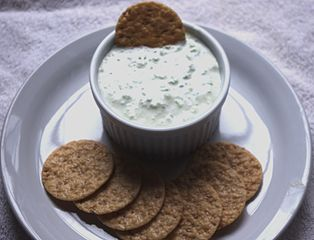
\includegraphics[width=10cm,height=10cm,keepaspectratio]{Figures/cheese.jpg}
\caption{Some cheese. Image Credit Geoff Lane (License: CC3-A-SA)}
\label{fig:CheeseFig}
\end{centering}
\end{figure}


\begin{figure}
\begin{centering}
\includegraphics[width=10cm,height=10cm,keepaspectratio]{Figures/dont-panic-e1534046233310.jpg}
\caption{The Hitch Hiker's Guide To The Galaxy (not to be confused with \cite{Reference1}. Image Credit David Strine (License: CC0)}
\label{fig:ThisFig}
\end{centering}
\end{figure}

%-----------------------------------
%	SUBSECTION 1
%-----------------------------------
\subsection{Subsection 1}

Nunc posuere quam at lectus tristique eu ultrices augue venenatis (Chapter \ref{chapter:firstchapter}).
Vestibulum ante ipsum primis in faucibus orci luctus et ultrices posuere cubilia Curae; Aliquam erat volutpat.
Vivamus sodales tortor eget quam adipiscing in vulputate ante ullamcorper.
Sed eros ante, lacinia et sollicitudin et, aliquam sit amet augue.
In hac habitasse platea dictumst (Section \ref{sec:firstsection}).

%-----------------------------------
%	SUBSECTION 2
%-----------------------------------

\subsection{Subsection 2}
Morbi rutrum odio eget arcu adipiscing sodales.
Aenean et purus a est pulvinar pellentesque.
 Cras in elit neque, quis varius elit.
 Phasellus fringilla, nibh eu tempus venenatis, dolor elit posuere quam, quis adipiscing urna leo nec orci.
 Sed nec nulla auctor odio aliquet consequat.
 Ut nec nulla in ante ullamcorper aliquam at sed dolor.
 Phasellus fermentum magna in augue gravida cursus.
 Cras sed pretium lorem.
 Pellentesque eget ornare odio.
 Proin accumsan, massa viverra cursus pharetra, ipsum nisi lobortis velit, a malesuada dolor lorem eu neque.

%----------------------------------------------------------------------------------------
%	SECTION 2
%----------------------------------------------------------------------------------------

\section{Main Section 2}

Sed ullamcorper quam eu nisl interdum at interdum enim egestas.
 Aliquam placerat justo sed lectus lobortis ut porta nisl porttitor.
 Vestibulum mi dolor, lacinia molestie gravida at, tempus vitae ligula.
 Donec eget quam sapien, in viverra eros.
 Donec pellentesque justo a massa fringilla non vestibulum metus vestibulum.
 Vestibulum in orci quis felis tempor lacinia.
 Vivamus ornare ultrices facilisis.
 Ut hendrerit volutpat vulputate.
 Morbi condimentum venenatis augue, id porta ipsum vulputate in.
 Curabitur luctus tempus justo.
 Vestibulum risus lectus, adipiscing nec condimentum quis, condimentum nec nisl.
 Aliquam dictum sagittis velit sed iaculis.
 Morbi tristique augue sit amet nulla pulvinar id facilisis ligula mollis.
 Nam elit libero, tincidunt ut aliquam at, molestie in quam.
 Aenean rhoncus vehicula hendrerit.

%\include{Chapters/Chapter2} 
%\include{Chapters/Chapter3}
%\include{Chapters/Chapter4} 
%\include{Chapters/Chapter5} 
%\include{Chapters/Chapter6}
%\include{Chapters/Chapter7}
%\include{Chapters/Chapter8}
%\include{Chapters/FavouriteChapter}

%----------------------------------------------------------------------------------------
%	THESIS CONTENT - APPENDICES
%----------------------------------------------------------------------------------------

\appendix % Cue to tell LaTeX that the following "chapters" are Appendices

% Include the appendices of the thesis as separate files from the Appendices folder
% Uncomment the lines as you write the Appendices

\include{Appendices/AppendixA}
%\include{Appendices/AppendixB}
%\include{Appendices/AppendixC}

%----------------------------------------------------------------------------------------
%	BIBLIOGRAPHY
%----------------------------------------------------------------------------------------

\printbibliography

\end{document}  
